\documentclass[portrait,a0,oldgerm]{a0poster}
\usepackage{ascmac}
\usepackage{amsmath}
\usepackage{bm}
\usepackage{bnf}
\usepackage[dvips]{graphicx,epsfig}
\usepackage{xcolor,lipsum}
\usepackage{multicol}
\usepackage{multirow}
%\usepackage{ulem}
%\usepackage{udline_euc}
\usepackage{wallpaper}
\setlength{\columnsep}{50pt}
\setlength{\fboxrule}{3pt}
\pagestyle{empty}
\def\thesection{\fontsize{46}{20}\selectfont \Roman{section}.}
\def\thesubsection{\fontsize{46}{20}\selectfont \roman{subsection}.}
\def\thesubsubsection{\fontsize{46}{20}\selectfont \roman{subsection}.\roman{subsubsection}.}
\def\baselinestretch{1.07}
\def\formularsize{\fontsize{60}{20}\selectfont}
\def\normalfontsize{\fontsize{36}{20}\selectfont}
\def\spaceV{\ \ \ \ \ }
\def\spaceX{\ \ \ \ \ \ \ \ \ \ }
\def\spaceXV{\ \ \ \ \ \ \ \ \ \ \ \ \ \ \ }
\def\spaceXX{\ \ \ \ \ \ \ \ \ \ \ \ \ \ \ \ \ \ \ \ }
\def\areaspace{9.4mm}
\def\ColoraTProCy{\color[cmyk]{0.7,0.7,0,0}}
\def\ColorbTAnaeroI{\color[cmyk]{1,0,1,0}}
\def\ColorcTAnaeroII{\color[cmyk]{0.5,0,0.5,0}}
\def\ColordTAnaeroIII{\color[cmyk]{0.2,0,0.2,0}}
\def\ColoreTAnfMethI{\color[cmyk]{1,0,0,0}}
\def\ColorfTAnfMethII{\color[cmyk]{0.4,0,0,0}}
\def\ColorgTPNifI{\color[cmyk]{0,1,1,0}}
\def\ColorhTPNifII{\color[cmyk]{0,0.7,0.7,0}}
\def\ColoriTPNifIII{\color[cmyk]{0,0.75,0,0}}
\def\ColorjTPNifIV{\color[cmyk]{0.5,1,0.5,0}}
\def\ColorkBK{\color[cmyk]{0,0,0,1}}
\def\waku{\color[cmyk]{0.2,0.5,0.7}}

\unitlength=1mm



\begin{document}
%%----- (* Wall Paper -----%%
%\TileWallPaper{11.7cm}{2cm}{Doshisha-n5.eps}
%%----- Wall Paper *) -----%%
%%----- (* space -----%%
\begin{center}
%\epsfig{file=WhiteSpace.ps,height=25mm}
\vspace{25mm}
\end{center}
%%----- space *) -----%%


%%----- (* Title -----%%
\begin{center}
\color[cmyk]{0,1,1,0.9}
\linespread{5.0}\fontsize{90}{20}\selectfont
tq :\\A Comprehensive Disciplinary Language for Materials Science
\end{center}
%%----- Title *) -----%%
%%----- (* Sub Title -----%%
%\begin{center}
%\color[cmyk]{1,1,0,0}
%\linespread{0.9}\fontsize{47}{20}\selectfont
%\end{center}
%%----- Sub Title *) -----%%
\vspace{20mm}
%%----- (* Author(s) and Affiliation(s) -----%%
\color[cmyk]{0,1,1,0.85}
\linespread{1.4}\fontsize{50}{20}\selectfont
\begin{center} \begin{tabular}[t]{ccc}
Kou Amano$^{\dag}$ &&Koichi Sakamoto$^{\dag}$ \\
\end{tabular} \end{center}
\color[cmyk]{0,1,1,0.82}
\linespread{1.4}\fontsize{48}{20}\selectfont
\begin{center} \begin{tabular}{c} 
$^\dag$Natinal Institute for Materials Science \\
\end{tabular} \end{center}
%%----- Author(s) and Affiliation(s) *) -----%%

\vspace{25mm}
\vspace{25mm}

%%----- (* Body, Single Column Region -----%%
%% Nothing
%%----- Body, Single Column Region *) -----%%
%%----- (* Body, Multi Column Region -----%%
%% color %%
%\definecolor{afb}{rgb}{0.8,0.85,0.9}
\color[cmyk]{1,1,0,0.8}
\begin{multicols}{3}
%%=====(* Col 1 =====%%
\noindent \noindent
\fcolorbox{orange}{white}{
\begin{minipage}[t]{242mm}
\vspace{5mm}\section*{\fontsize{48}{20}\selectfont No content} \vspace{-5mm}
\linespread{1.9}\fontsize{36}{20}\sffamily\selectfont
%%%%%%%%%% content %%%%%%%%%%
\vspace{5mm}
\end{minipage} }


\vspace{\areaspace} \noindent \noindent
\fcolorbox{orange}{white}{
\begin{minipage}[t]{242mm}
\vspace{5mm}\section*{\fontsize{48}{20}\selectfont Objective} \vspace{-5mm}
\linespread{1.9}\fontsize{36}{20}\sffamily\selectfont
tq should satisfy
\begin{itemize}
\color{black}\item parsing tree structure
\color{black}\item parsing graph structure
\color{gray}\item searching dictionary
\color{gray}\item matching terms using dictionary
\color{black}\item reforming from unstructured data to structured data
\color{black}\item conversion to other well-known formats such as JSON
\color{gray}\item matching or searching tree or graph structure
\color{gray}\item Term Rewriting by Network Similarity (TRNS)
\color{gray}\item daemonizing dictionary system
\color{gray}\item parallelizing.
\end{itemize}
\vspace{5mm}
\end{minipage} }


\vspace{\areaspace} \noindent \noindent
\fcolorbox{orange}{white}{
\begin{minipage}[t]{242mm}
\vspace{5mm}\section*{\fontsize{48}{20}\selectfont The language} \vspace{-5mm}
\subsection*{\fontsize{40}{20}\selectfont Short example} \vspace{0mm}
\linespread{1.9}\fontsize{36}{20}\sffamily\selectfont
%Short example:\\
%\\
\color{red}\#1\color{blue}\$Op\$\color{green}Name\color{black}(\color{magenta}\$\#1\color{cyan}[1]\color{black}) \\
$\downarrow$ tq in=/dev/stdin -FT -Pin data=test.csv\\
\color{red}\#1\color{blue}\$Op\$\color{green}Name\color{black}(\color{magenta}\$\#1\color{cyan}[1]\color{black}@@\color{brown}\#1\$Op\$Name\color{black}(\color{purple}Length\color{black})) \\
%\#1\$Op\$Name(\$\#1[1]@@\#1\$Op\$Name(Length))
\vspace{4mm}

\color{red}\#1 : $<label>$ \vspace{2mm}\\
\color{blue}\$Op\$ : $<operator>$ \vspace{2mm}\\
\color{green}Name : $<name>$ \vspace{2mm}\\
\color{magenta}\$\#1 : $<reference>$ \vspace{2mm}\\
\color{cyan}[1] : $<data \ bind \ dimension>$ \vspace{2mm}\\
\color{black}@@ : $<bind \ mark>$ \vspace{2mm}\\
\color{brown}\#1\$Op\$Name : $<binded \ object>$ \vspace{2mm}\\
\color{purple}Length : $<binded \ data>$\\
\\
\vspace{-30mm}
\color{black}\subsection*{\fontsize{40}{20}\selectfont Data structure} \vspace{0mm}
\ 
\\
\linespread{1.2}\fontsize{16}{20}\sffamily\selectfont
\begin{tabular}{llllllllllllllll}
\multicolumn{14}{c}{\fontsize{28}{20}\sffamily\selectfont Table: Members of the data structure}\\
&Lv&Adr&PAd&Ref&LT&LN&Hpt&H&D&VC&VSt&Cj&NC\\
\hline
0&0&14153344&0&0&h&1&2&\#1\$Op\$Name&&0&&0&1\\
1&1&14154608&14153344&14153344&&-1&0&\$\#1[1]&[1&1&Length&0&0\\
\end{tabular}
\vspace{5mm}
\end{minipage} }

%%===== Col 1 *)=====%%

%%=====(* Col 2 =====%%
\noindent \fcolorbox{orange}{white}{
\begin{minipage}[t]{242mm}
\vspace{5mm}\section*{\fontsize{48}{20}\selectfont Parsing} \vspace{-3mm}
\subsection*{\fontsize{40}{20}\selectfont Parsing tree}
\linespread{1.9}\fontsize{32}{20}\sffamily\selectfont
\color[cmyk]{0,0,0,1}
\begin{center}\begin{tabular}{lcl}
\vspace{70mm}Interpreted structure & & Statements \\
 & & Input: \\
 & & \ A(B(\#1C),\$\#1(D)) \\
 & & Output: \\
 & & \ A(B(\#1C),\$\#1@\#1C(D)) \\
\raisebox{\baselineskip}[0pt][0pt]{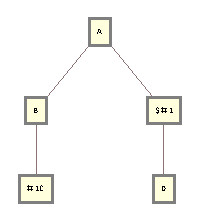
\epsfig{file=t1ig.eps,height=130mm}} & &  \\
\end{tabular}\end{center}
\color[cmyk]{1,1,0,0.8}

\subsection*{\fontsize{40}{20}\selectfont Parsing graph}
\vspace{5mm}
\linespread{1.9}\fontsize{32}{20}\sffamily\selectfont
\color[cmyk]{0,0,0,1}
\begin{center}\begin{tabular}{lcl}
\multicolumn{3}{c}{\textbf{Implicit graph}}\\
\vspace{28mm}Interpreted structure & & Statements \\
 & & Input:\\
 & & \ A(B(\#1C),\$\#1(D)) \\
 & & Adjacency matrix:\\
 & & \ [:A:0],1,2,3,,\\
 & & \ ,[:B:1],2,,,\\
 & & \ ,,[:\#1C:2],,,\\
 & & \ ,,,[:\$\#1:3$\rightarrow$2],4,\\
 & & \ ,,,,[:D:4],\\
\raisebox{\baselineskip}[0pt][0pt]{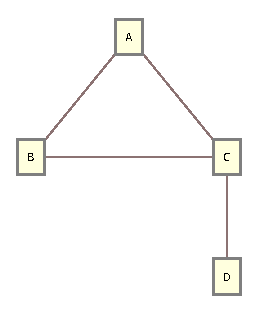
\epsfig{file=t2ig.eps,height=140mm}} & &  \\
\end{tabular}\end{center}

\vspace{5mm}
\begin{center}\begin{tabular}{lcp{100mm}}
\multicolumn{3}{c}{\textbf{Explicit graph}}\\
\vspace{7mm}Interpreted structure & & Statements \\
 & & \hspace{-3mm}Input:\\
 & & \linespread{1.2}\fontsize{20}{20}\sffamily\selectfont \$G\$(\$V\$(\#0,\#1,\#2), \$E\$(\$\#0(\$\#1,\$\#2), \$\#1(\$\#0,\$\#2), \$\#2(\$\#0,\$\#1)))\\
 & & \hspace{-3mm}Adjacency matrix:\\
 & & \linespread{1.2}\fontsize{20}{20}\sffamily\selectfont 
,,,3,4,,[:\$\#0:6$\rightarrow$2],7,8,,,,,,,
,,,,,,,[:\$\#1:7$\rightarrow$3],,,,,,,,
,,,,,,,,[:\$\#2:8$\rightarrow$4],,,,,,,
,,2,,4,,,,,[:\$\#1:9$\rightarrow$3],10,11,,,,
,,,,,,,,,,[:\$\#0:10$\rightarrow$2],,,,,
,,,,,,,,,,,[:\$\#2:11$\rightarrow$4],,,,
,,2,3,,,,,,,,,[:\$\#2:12$\rightarrow$4],13,14,
,,,,,,,,,,,,,[:\$\#0:13$\rightarrow$2],,
,,,,,,,,,,,,,,[:\$\#1:14$\rightarrow$3], \vspace{-10mm}\\
\raisebox{\baselineskip}[0pt][0pt]{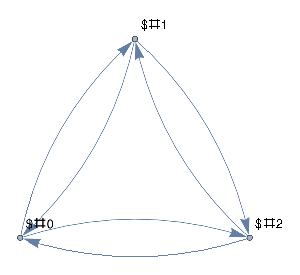
\epsfig{file=gr1.eps,height=120mm}} & &  \\
\end{tabular}\end{center}


\subsection*{\fontsize{40}{20}\selectfont Binding and reforming data} \vspace{-3mm}
\linespread{1.9}\fontsize{32}{20}\sffamily\selectfont
\color[cmyk]{0,0,0,1}
\begin{center}\begin{tabular}{lcp{100mm}}
\vspace{4mm}Interpreted structure & & Statements \\
 & & \hspace{-3mm}Input:\\
 & & \linespread{1.2}\fontsize{20}{20}\sffamily\selectfont (\#1\$1[2],\#2\$2[2],\$3[3](\#4\$4[2])); \$PI\$(\$\#1,Quantity(\$\#4,\$\#2)) \\
 & & \hspace{-3mm}Data:\\
 & & \linespread{1.2}\fontsize{20}{20}\sffamily\selectfont 
Length,Weight,
mm,kg,
1,2,
322,4,
5,68\\
 & & \hspace{-3mm}Output:\\
 & & \linespread{1.2}\fontsize{20}{20}\sffamily\selectfont (((Length,Quantity(1,mm)), (Weight,Quantity(2,kg))), ((Length,Quantity(322,mm)), (Weight,Quantity(4,kg))), ((Length,Quantity(5,mm)), (Weight,Quantity(68,kg)))) \vspace{-12mm}\\
\raisebox{\baselineskip}[0pt][0pt]{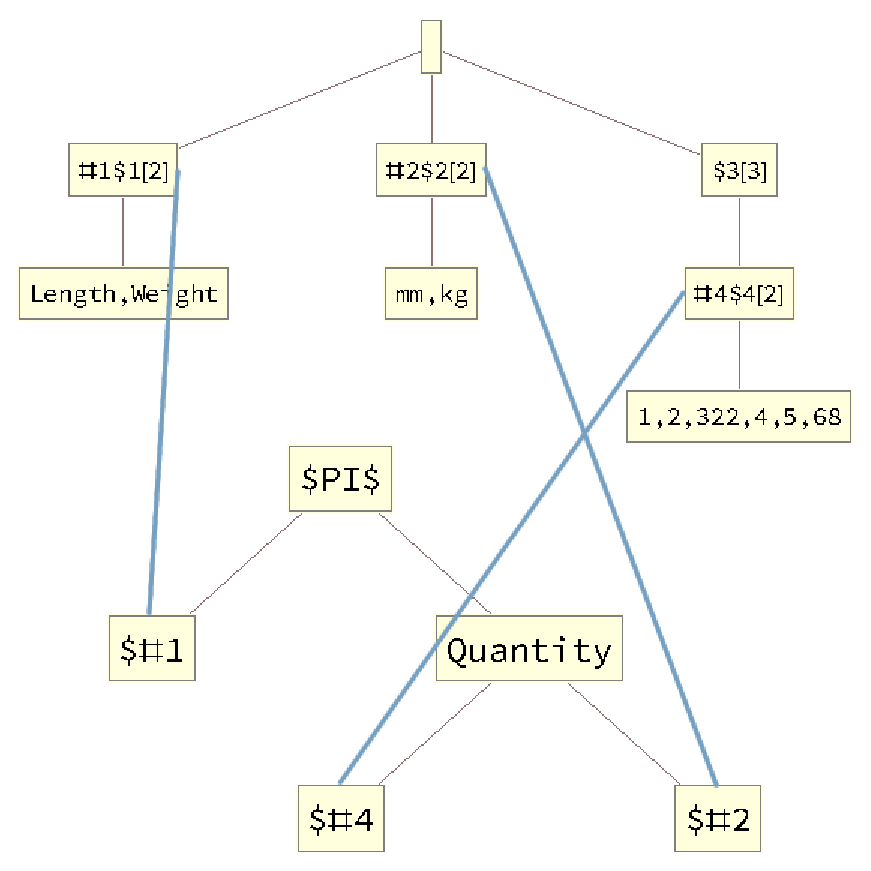
\epsfig{file=gdb2-2.eps,height=130mm}} & &  \\
%\raisebox{\baselineskip}[0pt][0pt]{\epsfig{file=gdb2-1.eps,height=110mm}} & &  \\
%\raisebox{\baselineskip}[0pt][0pt]{\epsfig{file=gdb2.eps,height=110mm}} & &  \\
%\raisebox{\baselineskip}[0pt][0pt]{\epsfig{file=fig-graph-bind.eps,height=110mm}} & &  \\
\end{tabular}\end{center}
\vspace{0.01mm}
\end{minipage} }


%%===== Col 2 *)=====%%

%%=====(* Col 3 =====%%
\noindent \fcolorbox{orange}{white}{
\begin{minipage}[t]{242mm}
\def\arraystretch{0.7}
\vspace{5mm}\section*{\fontsize{48}{20}\selectfont Development status} \vspace{-5mm}
\subsection*{\fontsize{40}{20}\selectfont Program construction} \vspace{0mm}
\linespread{1.9}\fontsize{36}{20}\sffamily\selectfont
\begin{itemize}
\item tq parser (designated as "tq") ... Done
\item converter ... Developing
\item analyzer ... TBD
\end{itemize}

\color[cmyk]{1,1,0,0.8}
\subsection*{\fontsize{40}{20}\selectfont Supported forms} \vspace{3mm}
\linespread{1.9}\fontsize{36}{20}\sffamily\selectfont
\color[cmyk]{0,0,0,1}

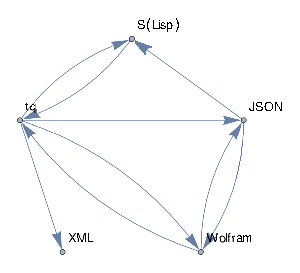
\epsfig{file=convg.eps,height=160mm}


\subsection*{\fontsize{40}{20}\selectfont Performance} \vspace{0mm}
\linespread{2.1}\fontsize{28}{20}\sffamily\selectfont
\color[cmyk]{0,0,0,1}
\begin{center}
\begin{tabular}{lrrr}
\multicolumn{4}{c}{Table: Parsing performance @ E5-2650} \\
Program & Size (nodes) & Time (min:sec) & Memory (bytes) \\
\hline
\hline
tq (stable) & 124,653,854 & 45 & 26G \\
tq (exptl.) & 124,653,854 & 27 & 12G \\
jq & 124,653,854 & 2:25 & 36G \\
\hline
tq (stable) & 498,615,417 & 3:30 & 104G \\
tq (exptl.) & 498,615,417 & 1:55 & 51G \\
jq & 498,615,417 & 10:50 & 144G \\
\end{tabular}
\end{center}

\linespread{2.1}\fontsize{28}{20}\sffamily\selectfont
\color[cmyk]{0,0,0,1}
\begin{center}
\begin{tabular}{lrrr}
\multicolumn{4}{c}{Table: Parsing and converting performance} \\
Form & Size (nodes) & Time (min:sec) & Memory (bytes) \\
\hline
\hline
JSON & 124,653,854 & 1:21 & 29G \\
JSON & 498,615,417 & 5:35 & 136G \\
\end{tabular}
\end{center}
\vspace{1mm}
\end{minipage} }


\vspace{\areaspace} \noindent \noindent
\fcolorbox{orange}{white}{
\begin{minipage}[t]{242mm}
\vspace{5mm}\section*{\fontsize{48}{20}\selectfont Future plan} \vspace{-5mm}
\linespread{1.9}\fontsize{36}{20}\sffamily\selectfont
%%%%%%%%%% content %%%%%%%%%%
\ As a next step, we are restructuring the data structure of tq for parallelizing. In the current structure, the tree structure and node property are strongly related; therefore, parallelizing is difficult. We are attempting to divide the data structure into tree structure and node table.

\vspace{5mm}
\end{minipage} }


\vspace{\areaspace} \noindent \noindent
\fcolorbox{orange}{white}{
\begin{minipage}[t]{242mm}
\vspace{5mm}\section*{\fontsize{48}{20}\selectfont Conclusion} \vspace{-5mm}
\linespread{1.9}\fontsize{36}{20}\sffamily\selectfont
%%%%%%%%%% content %%%%%%%%%%
\ tq can handle various types of data in a uniform manner, especially in the field of materials science.
Adopting the syntax of S-expressions, tq incorporates the binding and node referencing mechanism to represent a graph structure that defines input and output data formats.
Due to its expressive power, users can write a set of rules that reform unstructured data (e.g.CSV) into those of an arbitrary format as they need, such as a tensor format for machine learning.

\vspace{5mm}
\end{minipage} }

%%===== Col 3 *)=====%%

\end{multicols}
%%----- Body, Multi Column Region *) -----%%

%%----- (* Body, Single Column Region -----%%
%% Nothing
%%----- Body, Single Column Region *) -----%%

\vspace{17mm}

%%----- (*  Logo -----%%
\begin{center}
%%\begin{tabular}{ccccccc}
%\begin{tabular}{ccccc}
%\epsfig{file=Tsukuba-Univ-mark200.eps,height=50mm} &
%\spaceV &
%%\epsfig{file=nias_logo.ps,height=50mm} &
%\spaceV &
%\epsfig{file=riken_g.eps,height=50mm} \\
%\end{tabular}
%\epsfig{file=KAKEN_logo.eps,height=35mm}
\end{center}
%%-----  Logo *) -----%%



%%----- (* For print all image -----%%
\begin{center}
%\epsfig{file=WhiteSpace.ps,height=25mm}
\vspace{25mm}
\end{center}
%%----- For print all image *) -----%%

\end{document}
